% ----------------------------------------------------------------------------------------\
% ---------------------------------------------------------------------------------------\
% --------------------------------------------------------------------------------------\
\section{Desarrollo}
% ----------------------------------------------------------------------------------------\
% ---------------------------------------------------------------------------------------\
% --------------------------------------------------------------------------------------\
% Explicación de las implementaciones, diagrama de flujo, ideas, comentarios, investigación, etc
% ----------------------------------------------------------------------------------------\
% ---------------------------------------------------------------------------------------\
\subsection{Implementación básica del Juego de la Vida}
% ----------------------------------------------------------------------------------------\
% ---------------------------------------------------------------------------------------\
El Juego de la vida es un autómata celular, es decir es un modelo matemático llevado de manera computacional para observar de manera dinámica cómo evoluciona en el tiempo. Creado por John Horton Conway en 1969 que consiste en una cuadrícula donde se marcan o desmarcan siendo pintados por un color, representando células y reflejando si esta se encuentra viva o muerta.


Iniciado el juego son las reglas las que determinan como acaba. El objetivo es crear un sistema que simulase la vida y su naturaleza. La manera en que se logra es con el nacimiento y supervivencia de estos seres binarios digitales donde depende del número de vecinos que estén a su vez vivos o muertos. Por lo que es posible observar patrones complejos e impredecibles gracias a unas sencillas reglas. Siendo utilizado como un modelo de simulación para estudiar fenómenos biológicos, evolutivos o físicos.

\begin{figure}[H]
    \centering
    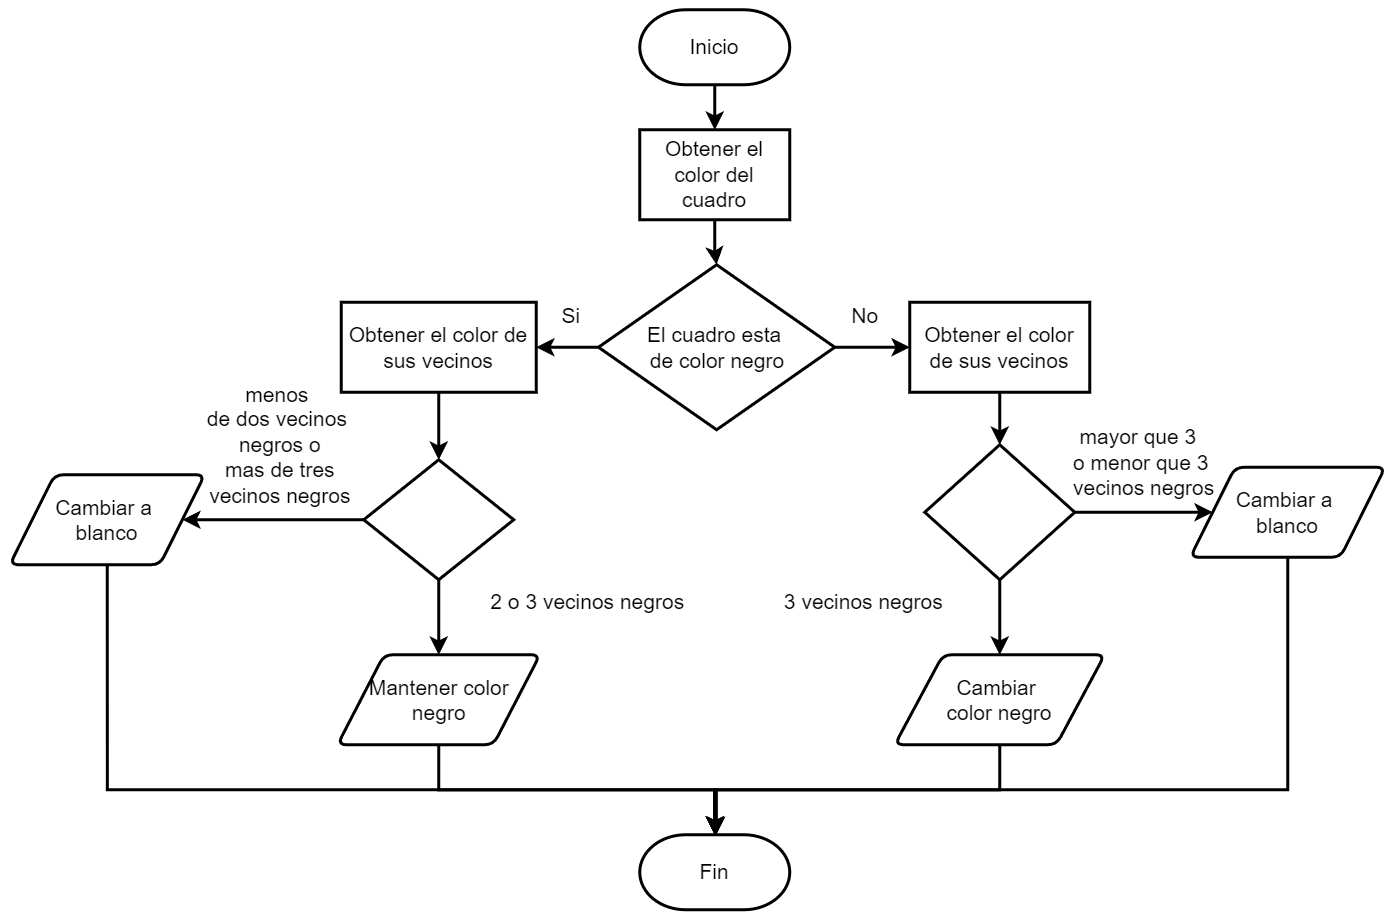
\includegraphics[width=0.9\linewidth]{IMA/DiagramaFlujoJuegoLaVida.png} 
    \caption{Diagrama de flujo del Juego de la Vida} 
\end{figure}

En el diagrama se puede observar las reglas que se siguen para determinar si una célula vive o muere.
En este caso las condicionales del diagrama reflejan la sobrepoblación, la soledad , la reproducción y la supervivencia de las células.
Por lo que solo faltaria implementar el código en Python para poder visualizar el juego de la vida.


% ----------------------------------------------------------------------------------------\
% ---------------------------------------------------------------------------------------\
\subsection{Introducción a los Algoritmos Genéticos}
% ----------------------------------------------------------------------------------------\
% ---------------------------------------------------------------------------------------\




% ----------------------------------------------------------------------------------------\
% ---------------------------------------------------------------------------------------\
\subsection{Implementación de Algoritmos Genéticos en el Juego de la Vida}
% ----------------------------------------------------------------------------------------\
% ---------------------------------------------------------------------------------------\